\section{Лекция 14.06.2018}

$V$ -- векторное пространство над $F$

$\varphi: V \rightarrow V$ -- линейный оператор

$\chi_{\varphi} (t) = (t - \lambda_1)^{k_1} \dots (t - \lambda_s)^{k_s}$

$i \in \{1, \dots, s\} \Rightarrow V^{\lambda_i} (\varphi)$ -- корневое подпространство

$dim V^{\lambda_i} (\varphi) = k_i$

$V = V^{\lambda_1} (\varphi) \oplus \dots \oplus V^{\lambda_s} (\varphi)$

$\varphi_i = (\varphi - \lambda_i \cdot Id) | _{V^{\lambda_i} (\varphi)}$

$Spec \varphi_i = \{0\}$

$\varphi_i^{k_i} = 0$

\bigskip
\textbf{Определение.} Линейный оператор $\varphi$ называется \textit{нильпотентным}, если $\exists \ m \in \NN$, такой что $\varphi^m > 0$.

\bigskip
Пусть $m \in \NN$ наименьшее с таким свойством.

$\{0\} = Ker \varphi \subsetneqq Ker \varphi^1 \subsetneqq Ker \varphi^2 \subsetneqq \dots \subsetneqq Ker \varphi^m = V$

$d_i = dim Ker \varphi^i$

$0 = d_0 < d_1 < d_2 < \dots < d_m = n = dim V$

$v \in V, ht(v) = k$

\bigskip
\textbf{Лемма.} Векторы $v, \varphi(v), \dots, \varphi^{k-1}(v)$ линейно независимы.

\bigskip
$C(v) = <v, \varphi(v), \dots, \varphi^{k-1} (v)>$

\bigskip
\textbf{Определение.} $C(v)$ называется \textit{циклическим подпространством}, порожденным вектором $v$.

\bigskip
$C(v) \ \varphi$-инвариантно

\bigskip
$B(v) = (\varphi^{k-1} (\varphi), \dots, \varphi(v), v)$ -- базис в $C(v)$

\bigskip
Матрица линейного оператора $\varphi|_{C(v)}$ в базисе $B(v)$ равна \begin{equation*}\begin{pmatrix} 0 & 1 & 0 & \dots & 0 & 0 \\ 0 & 0 & 1 & \dots & 0 & 0 \\ 0 & 0 & 1 & \dots & 0 & 0 \\ \vdots & \vdots & \vdots & \ddots & \vdots & \vdots \\ 0 & 0 & 0 & \dots & 0 & 1 \\ 0 & 0 & 0 & \dots & 0 & 0 \\ \end{pmatrix}\end{equation*}

Вывод: достаточно разложить $V$ в прямую сумму циклических подпространств.

\subsection{Метод построения жорданова базиса}

\bigskip
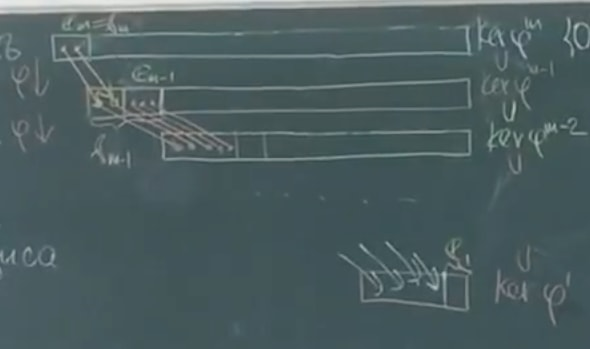
\includegraphics[width=10cm,height=15cm,keepaspectratio]{example7.jpg}

\bigskip
\underline{Шаг 1.} Выберем линейно независимый набор $e_m \subseteq Ker \varphi^m$, такой что $Ker \varphi^m = <e_m> \oplus Ker \varphi^{m-1}$

Положим $f_m = e_m$

\bigskip
\underline{Шаг 2.} Выберем линейно независимый набор $e_{m - 1} \subseteq Ker \varphi^{m-1}$, такой что $Ker \varphi^{m-1} = <\varphi(f_m)> \oplus <e_{m-1}> \oplus Ker \varphi^{m-2}$

Положим $f_{m-1} = \varphi(f_m) \cup e_{m-1}$

\bigskip
(и так далее)

\bigskip
\underline{Шаг $m$.} Выберем линейно независимый набор $e_1 \subseteq Ker \varphi$, такой что $Ker \varphi = <\varphi(f_2)> \oplus <e_1>$

\bigskip
На выходе получаем наборы $e_m, \dots, e_1$

Положим $e = e_m \cup \dots \cup e_1$

\bigskip
\textbf{Теорема.} 1) $V = \oplus_{e' \in e} C(e')$

2) $\cup_{e' \in e} B(e')$ -- жорданов базис для $\varphi$

\bigskip
Пусть $c_k$ число жордановых клеток размера $k$

$c_k = |e_k|$

$Ker \varphi^k = <\varphi(f_{k+1})> \oplus <e_k> \oplus Ker \varphi^{k-1}$

$d_k = \overbrace{|\varphi(f_{k+1})|}^{= d_{k+1} - d_k} + c_k + d_{k-1}$

$d_k = d_{k+1} - d_k + c_k + d_{k - 1}$

$c_k = 2d_k - d_{k-1} - d_{k+1}$

\subsection{Полуторалинейные формы и эрмитовы пространства}

\bigskip
билинейная форма

$\downarrow$

симметричная билинейная форма

$\downarrow$

квадратичная форма

$\downarrow$

положительно определенная квадратичная форма (над $\RR$)

$\downarrow$

евклидово пространство (над $\RR$)

\bigskip
\textbf{Определение.} \textit{Полуторалинейная форма (1,5-линейная)} на векторном пространстве $V$ над $\CC$ -- это отображение $\beta: V \times V \rightarrow \CC$, такое что

1) Полулинейность по первому аргументу

$\beta(\alpha_1 x_1 + \alpha_2 x_2, y) = \overline{\alpha_1} \beta (x_1, y) + \overline{\alpha_2} \beta (x_2, y)$

2) Линейность по второму аргументу

\bigskip
В координатах $x = \begin{pmatrix} x_1 \\ \vdots \\ x_{n} \end{pmatrix}, y = \begin{pmatrix} y_1 \\ \vdots \\ y_{n} \end{pmatrix}$

$\beta(x, y) = (\overline{x_1}, \dots, \overline{x_n}) B \begin{pmatrix} y_1 \\ \vdots \\ y_{n} \end{pmatrix}$

\bigskip
Формула изменения матрицы 1,5-линейной формы:

$B' = C^* B C$

$C^* = \overline{C}^T = (\overline{c_{ji}})$

\bigskip
\textbf{Определение.} 1,5-линейная форма называется \textit{эрмитовой}, если $\beta(y, x) = \overline{\beta(x, y)}$

\bigskip
$\beta(x, x) = \overline{\beta(x, x)} \Rightarrow \beta(x, x) \in \RR$

$Q(x) = \beta(x, x)$ -- эрмитова квадратичная форма

\bigskip
$Q:V \rightarrow R$

\textbf{Теорема о нормальном виде.} $Q$ -- эрмитова квадратичная форма $\Rightarrow \exists$ базис, такой что $Q(x) = |x_1|^2 + \dots + |x_k|^2 - |x_{k+1}|^2 - \dots - |x_{k + s}|^2$

\bigskip
\textbf{Определение.} \textit{Эрмитово пространство} -- это векторное пространство над $\CC$, на котором задано скалярное произведение, то есть положительно определенная эрмитова 1,5-линейная форма.

\bigskip
1,5-линейная форма

$\downarrow$

эрмитова форма

$\downarrow$

эрмитова квадратичная форма

$\downarrow$

положительно определенная эрмитова квадратичная форма (над $\CC$)

$\downarrow$

эрмитово пространство (над $\CC$)

\bigskip
Длина: $|x| = \sqrt[]{(x, x)}$

Неравенство Коши-Буняковского

Неравенство треугольника

Ортогональность

Ортогональное дополнение

$U$ -- подпространство в $V \Rightarrow V = U \oplus U^{\bot}$

Ортонормированный базис

\bigskip
$e, e'$ -- два ортогональных базиса, $e' = e \cdot C$

$C$ -- унитарная матрица

$C^{-1} = C^*$

\bigskip
\textbf{Линейный операторы в эрмитовых пространствах}

1) самосопряженный $(\varphi(x), y) = (x, \varphi(y))$

2) унитарный $(\varphi(x), \varphi(y)) = \varphi(x, y)$

\bigskip
\textbf{Теорема.} 1) $\varphi$ -- самосопряженный $\Rightarrow \exists$ ортонормированный базис из собственных векторов; $Spec \varphi \subseteq \RR$

2) $\varphi$ -- унитарный оператор $\Rightarrow \exists$ ортонормированный базис из собственных векторов

$\lambda \in Spec f \Rightarrow |\lambda| = 1$

\bigskip
Аналогичное сингулярное разложение

\bigskip
$A \in Mat_{m \times n} (\CC) \Rightarrow \exists$ унитарная матрица $U \in M_m(\CC), V \in M_n (\CC)$, такие что $A = U \Sigma V^*$

$\Sigma = \begin{pmatrix} \sigma_1 & 0 & 0 & 0 & 0 & 0 & 0 \\  0 & \sigma_2 & 0 & 0 & 0 & 0 & 0 \\ 0 & 0 & \ddots & 0 & 0 & 0 & 0 \\ 0 & 0 & 0 & \sigma_r & 0 & 0 & 0 \\ 0 & 0 & 0 & 0 & 0 & 0 & 0 \\ 0 & 0 & 0 & 0 & 0 & \ddots & 0 \\ 0 & 0 & 0 & 0 & 0 & 0 & 0 \end{pmatrix}, \sigma_i \in \RR, \sigma_1 \geqslant \dots \geqslant \sigma_r > 0, \sigma_i$ определено однозначно 























\end{document}